\section{Примеры неустойчивых стационарных решений}

Приведем численные примеры, демонстрирующие зависимость устойчивости
стационарного решения \eqref{shock_like} от параметра $\tau > 0$ и от
"возмущающих" гармоник $\theta_0$ (под гармоникой функции $\theta_0$ понимается
соответствующий компонент ряда Фурье в разложении $\theta_0$ по базису в $H$.
\newtheorem{exmp_bur}{Пример}
\begin{exmp_bur}
\end{exmp_bur}

Начальное условие $\theta_0(x) = \frac{\sin(\pi x)}{G(x)}$, параметр $\tau$ 
возмем равный 15. На рис. 7 показано неустойчивое поведение системы
\eqref{fluct}

\begin{figure}[h]
    \centering
    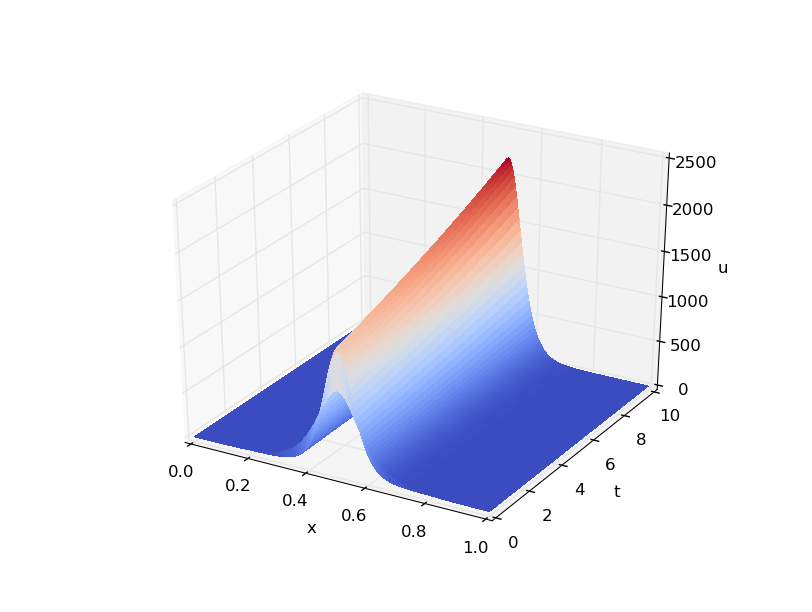
\includegraphics[width=3.0in]{ex_s15}
    \caption{}
    \label{fig:fig07}
\end{figure}

\begin{exmp_bur}
\end{exmp_bur}
Начальное условия $\theta_0(x) = \frac{x^2}{G(x)}$. Параметр $\tau = 15$.
Поведение решения представлено на рис.8.

\begin{figure}[h]
    \centering
    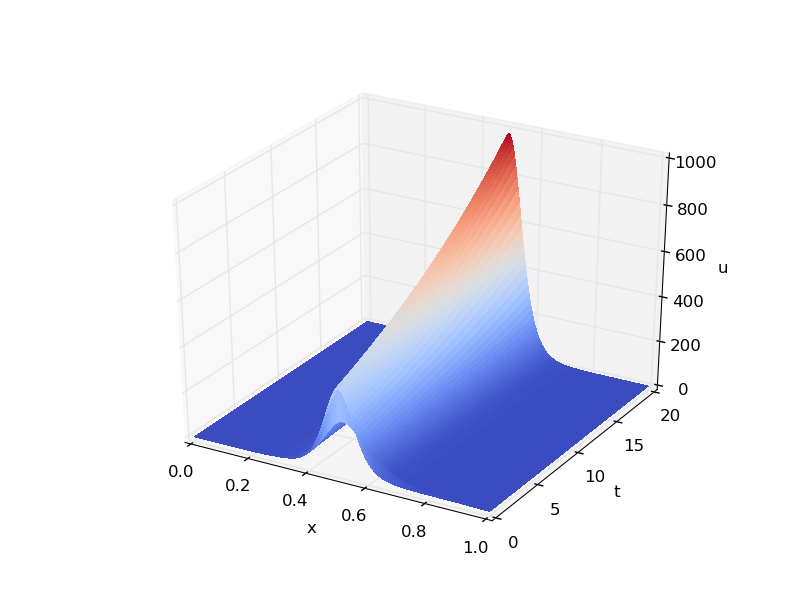
\includegraphics[width=3.0in]{ex_x2_s15}
    \caption{}
    \label{fig:fig08}
\end{figure}
